\documentclass[
	12pt,				% tamanho da fonte
	openright,			% capítulos começam em pág ímpar (insere página vazia caso preciso)
	twoside,			% para impressão em recto e verso. Oposto a oneside
	a4paper,			% tamanho do papel.
	chapter=TITLE,		% títulos de capítulos convertidos em letras maiúsculas
	section=TITLE,		% títulos de seções convertidos em letras maiúsculas
	sumario=abnt-6027-2012,
	english,			% idioma adicional para hifenização
	brazil				% o último idioma é o principal do documento
]{abntex2}
\usepackage{import}    % package import tem o comando import que faz a importação com "novo path"
\usepackage{packages/udescCCT} 	% Pacote de customizações da UDESC/CCT

\import{0-conf/}{!main}

% -----------------------------------------------------------------
% Informações de dados para CAPA e FOLHA DE ROSTO
% -----------------------------------------------------------------
\tipotrabalho{Atividade prática como componente curricular}
\titulo{Observações e análise sociológica reflexiva das relações entre a sociedade e o meio ambiente}%
% ATENÇÃO: O símbolo {} indica o sobrenome para a ficha catalográfica.
% Exemplo: Sherlock Holmes {}da Silva para sobrenomes compostos;
% Exemplo: Arnold Alois {}Schwarzenegger para sobrenome simples.
\autor{Francisco Lima {}Figueiredo}%
\orientador{Fernando de {}Figueiredo Balieiro}%
\coorientador{Daniel Tadeu {}do Amaral}%
\instituicao{Universidade Estácio de Sá}%
\preambulo{Trabalho apresentada ao professor Daniel Tadeu do Amaral como parte dos trabalhos a serem apresentados na disciplina ASPECTOS ANTROPOLÓGICOS E SOCIOLÓGICOS DA EDUCAÇÃO (CEL0466/3521060 - 9011).}
\local{Brasília}%
\data{\the\year}%
% ---

% compila o indice
\makeindex

% -----------------------------------------------------------------
% Início do documento
% -----------------------------------------------------------------
\begin{document}
	\import{1-pream/}{!main}


    % -----------------------------------------------------------------
    % ELEMENTOS TEXTUAIS
    % -----------------------------------------------------------------
    \textual

    % Mantenha está estrutura, assim você deixa o trabalho mais organizado

    \chapter{Objetivos}

    \chapter{Introdução Teórica}

Não é possível entrar no tema \textbf{Meio Ambiente} sem mencionar a Educação Ambiental nas escolas, uma vez que esperamos que nossas crianças evoluam com uma mentalidade melhor que a nossa no tocante ao meio ambiente.\\

\citeonline{Dias1994}  diz que a "Educação Ambiental se caracteriza por
incorporar as dimensões sociais, políticas, econômicas,
culturais, ecológicas e éticas, deixando claro que ao discutir
qualquer problema ambiental é fundamental a consideração
de todos estes aspectos." Segundo este autor, "a maior parte
dos problemas ambientais tem suas raízes na miséria que,
por sua vez, é gerada por políticas e problemas econômicos,
concentradores de riqueza e responsáveis pelo desemprego
e degradação ambiental."\\

Pode-se também definir a educação ambiental, nas palavras de \citeonline{Magalhaes2018}, como um processo
onde o educando obtém conhecimentos acerca das
questões ambientais e assim passa a ter um novo
entendimento acerca do meio ambiente, se tornando um
agente transformador referente à preservação do meio
ambiente e de seus recursos naturais. \\

\citeonline{Gadotti2000} explica que educação ambiental vai muito além do conservacionismo
Trata-se de uma mudança radical de mentalidade em
relação à qualidade de vida, que está diretamente ligada
ao tipo de convivência que mantemos com a natureza e
que implica em atitudes, valores, ações. Trata-se de uma
opção de vida por uma relação saudável e equilibrada,
com o contexto, com os outros, com o ambiente mais
próximo, a começar pelo ambiente de trabalho e
doméstico.\\

\section{Contexto Geográfico: Brasília}

Brasília foi inaugurada em 21 de abril de 1960

\newacronym{CODEPLAN}{CODEPLAN}{Companhia de Planejamento do Distrito Federal }

De acordo com o \citeonline{CODEPLANSEPLAN2013}

\begin{figure}[h]
    \centering
    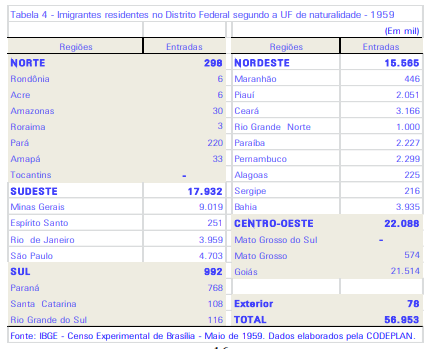
\includegraphics[width=0.7\linewidth]{fig/imigrantes-1959}
    \label{fig:imigrantes-1959}
    \caption{Imigrantes residentes no DF em 1959}
\end{figure}

\lipsum[1-30]

\begin{figure}[h]
    \centering
    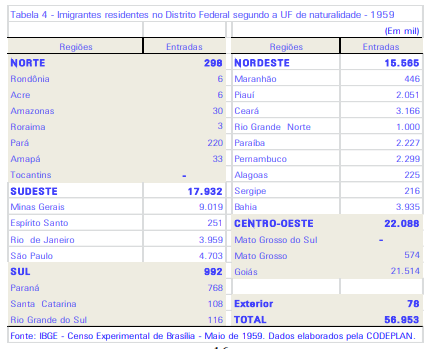
\includegraphics[width=0.7\linewidth]{fig/imigrantes-1959}
    \caption{}
%    \label{fig:imigrantes-1959}
\end{figure}

\begin{figure}[h]
    \centering
    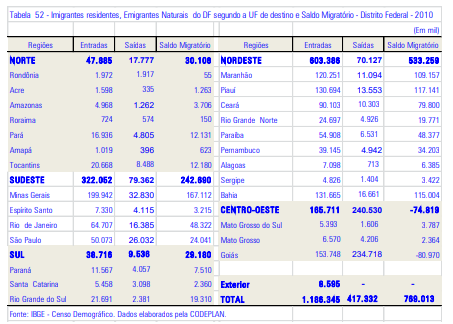
\includegraphics[width=0.7\linewidth]{fig/imigrantes-2010}
    \caption{}
    \label{fig:imigrantes-2010}
\end{figure}

    \chapter{Procedimentos Metodológicos}

Teste
    \chapter{Resultados e Conclusão}

Nas palavras de \cite{Magalhaes2018} "A educação ambiental impacta não apenas no meio em que vivemos, mas está diretamente ligada à
sobrevivência humana, e precisa estar presente no ensino de forma incisiva.
A introdução da educação ambiental nos primeiros anos da educação infantil potencializa o
processo de ensino-aprendizagem, uma vez que o ambiente escolar é um dos meios de integração e
conscientização mais completos para abordar as problemáticas entre a relação homem e natureza.
Quando a educação ambiental é aplicada desde o início do processo de educação e se torna
constante nos anos subsequentes, a aprendizagem transforma-se permanentemente.
É evidente que as mudanças no meio ambiente ocorrem de forma lenta e gradativa, mas quanto
antes iniciado o processo de educação e conscientização da população, maiores são as chances de
sucesso. Assim, é de fato extremamente importante que a Educação Ambiental seja inserida desde
os primeiros anos da educação infantil.
Entretanto, este não é um dever apenas da escola: é fundamental que todos os segmentos da
sociedade em que a criança está inserida se envolvam e busquem este objetivo comum. Está
conscientização das crianças também é um dever dos pais e da sociedade em geral."\\




    % -----------------------------------------------------------------
    % ELEMENTOS PÓS-TEXTUAIS
    % -----------------------------------------------------------------
    \postextual

    % Você pode comentar os elementos que não deseja em seu trabalho;

    % Referências bibliográficas
    %\bibliography{PosTextuais/Biblio-Trab0001}	    % Elemento Obrigatório
    \bibliography{PosTextuais/Biblio-Trab0001}	    % Elemento Obrigatório

    % ----------------------------------------------------------
% Glossário
% ----------------------------------------------------------

Consulte o manual da classe abntex2 para orientações sobre o glossário.

\makeglossaries
			    % Elemento Opcional
    
% ----------------------------------------------------------
% Apêndices
% ----------------------------------------------------------

% ---
% Inicia os apêndices
% ---
\begin{apendicesenv}

% Imprime uma página indicando o início dos apêndices
\partapendices

% ----------------------------------------------------------
\chapter{Quisque libero justo}
% ----------------------------------------------------------

\lipsum[50]

% ----------------------------------------------------------
%\chapter{Nullam elementum urna vel imperdiet sodales elit ipsum pharetra ligula
%ac pretium ante justo a nulla curabitur tristique arcu eu metus}
%% ----------------------------------------------------------
%\lipsum[55-57]

\end{apendicesenv}
% ---				% Elemento Opcional
    
% ----------------------------------------------------------
% Anexos
% ----------------------------------------------------------
%
% ---
% Inicia os anexos
% ---
\begin{anexosenv}

% Imprime uma página indicando o início dos anexos
\partanexos

% ---
\chapter{Morbi ultrices rutrum lorem.}
% ---
\lipsum[30]

% ---
%\chapter{Cras non urna sed feugiat cum sociis natoque penatibus et magnis dis
%parturient montes nascetur ridiculus mus}
%% ---
%
%\lipsum[31]
%
%% ---
%\chapter{Fusce facilisis lacinia dui}
%% ---
%
%\lipsum[32]

\end{anexosenv}
				% Elemento Opcional
    %
%%---------------------------------------------------------------------
%% INDICE REMISSIVO
%%---------------------------------------------------------------------
\phantompart
\printindex
%---------------------------------------------------------------------

		% Elemento Opcional

\end{document}

% -----------------------------------------------------------------
% Fim do Documento
% -----------------------------------------------------------------